\documentclass{beamer}
\usepackage{tikz}

\usepackage{graphicx}
\usepackage[spanish]{datetime2}
\usepackage[spanish]{babel}
\usepackage{hhline}
\usepackage{epstopdf}
\usepackage{diagbox}
\usepackage{subcaption}

\usetheme{Madrid}
\definecolor{blmblue}{HTML}{003366}  % Granate UDC d2007b
\setbeamercolor{structure}{fg=blmblue} % Aplicar el color BLM a la estructura

\setbeamertemplate{navigation symbols}{}

\title[Trabajo Fin de Grado]{Perfilado automático de usuarios en corpus sociales sobre el movimiento \textit{Black Lives Matter}}
\author{Nicolás Míguez García}
\institute[GEI]{Grado en Ingeniería Informática (Mención en Computación) \\
	\vspace{3mm}
	Patricia Martín Rodilla \\ 
	David Otero Freijeiro 
} 

\date[\today]{}

\addtobeamertemplate{title page}{
	\begin{tikzpicture}[remember picture,overlay]
		\node[anchor=west,xshift=9pt,yshift=-8cm] at (current page.north west) {
\includegraphics[scale=0.05]{Logo_fic.jpg}}; 
		\node[anchor=east,xshift=-3.5pt,yshift=-8.5cm] at (current page.north east) {
\includegraphics[scale=0.12]{udc.png}};
	\end{tikzpicture}
}

\begin{document}
	
	\frame{\titlepage}
%	\begin{frame}
%	\end{frame}
		
	\AtBeginSection[]
	{
		\begin{frame}<beamer>
			\frametitle{Índice general}
			\tableofcontents[currentsection]
		\end{frame}
	}
\section{Motivación y objetivos}
		\begin{frame}
			\frametitle{Motivación}
			\begin{itemize}
				\item Las RRSS han cambiado el modo de vida actual convirtiéndose uno de los principales medios de debate y difusión de información.
				\item La recopilación de textos y publicaciones de estas, ha dado lugar a la creación de 'archivos sociales', para la documentación de ciertos procesos.
				\item Con motivo de las protestas raciales surgidas en 2020 acerca del movimiento \textit{Black Lives Matter} (\textbf{\#BLM}) se ha creado una colección de referencia.
				\item Contiene +260.000 publicaciones de +90.00 usuarios de \emph{Reddit} en inglés y español.
				\item Para el estudio del subconjunto en \emph{español} se ha propuesto este TFG.
			\end{itemize}
		\end{frame}
		
		\begin{frame}
			\frametitle{Objetivos}
			\begin{definition}[Author profiling]
				Se conoce como \textbf{perfilado de usuarios} al procesamiento y análisis de textos para la identifiación de atributos como género o edad acerca de los mismo.
			\end{definition}
			\begin{itemize}
				\item Estudio del estado del arte del \textit{author profiling} en materia de género y edad sobre textos en \textbf{español}.
				\item Comparación, selección e implementación de los algoritmos con mejor rendimiento.
				\item Construcción de un \textit{dashboard} web para el perfilado y visualización de collecciones de usuarios.
				\item Estudio de resultados de perfilado sobre colección \#BLM.
			\end{itemize}
		\end{frame}
		
\section{Fundamentos}
		
		\subsection{Estado del arte}
		\begin{frame}
			\frametitle{Fundamentos}
			\framesubtitle{Estado del arte}
			\begin{itemize}
				\item El interés por el perfilado de usuarios se vió patente con algunos trabajos tempranos basados en blogs en inglés (2006 y 2007).%(Argamon et al,. en 2007 y Scheler et al. en 2006).
				\item Competiciones PAN organizadas por el grupo Webis:
				Perfilado de usuarios para género y edad, textos de Twitter y Blogs en español (2013 - 2016).
				\item Competiciones IberLEF (exclusivamente en español) organizadas por la SEPLN.
				perfilado de género e ideología política de usuarios en Twitter (2022).
				\item Estas proporcionaron los conjuntos de datos y algortimos a emplear en nuestro problema.
			\end{itemize}
		\end{frame}
		\subsection{Cojuntos de datos}
		\begin{frame}
			\frametitle{Fundamentos}
			\framesubtitle{Conjuntos de datos}
			\begin{table}[hp!]
				\centering
				\begin{tabular}{|l|ll|l|l|}
					\hhline{~---~}
					\multicolumn{1}{c|}{} & \multicolumn{2}{c|}{\textbf{PAN-AP 2015}} & \textbf{PAN-AP 2016} & \multicolumn{1}{c}{}\\ \hline
					Categoría & Training & Test & Training & Total\\ \hline
					18-24 & 22 & 18 & 11 & 51\\
					25-34 & 46 & 44 & 54 & 144\\
					35-49 & 22 & 18 & 116 & 156\\
					+50 & 10 & 8 & 41 & 59\\ \hline
					Hombres & 50 & 44 & 111 & 204\\
					Mujeres & 50 & 44 & 111 & 204\\ \hline
					Total & 100 & 88 & 222 & 410\\ \hline  
				\end{tabular}%
				\caption{Distribución de usuarios en función de edad y género en los conjuntos de entrenamiento utilizados.}
				\label{tab:datasets_edad}
			\end{table}
		\end{frame}
		
%		\begin{frame}
%			\frametitle{Algoritmos de perfilado}
%			\framesubtitle{1ª aproximación}
%			\begin{itemize}
%				\item Ganador IberLef 2022 (ideología política).
%				\item  Red neuronal basada en \textit{transformers}.
%				\item \textit{Embeddings} de BETO y MarIA.
%				\item Entrenamiento y uso costosos (TPU).
%				\item Peor rendimiento de los tres.
%				\item Requiere + datos de entrenamiento.
%
%			\end{itemize}
%		\end{frame}
%		
%		\begin{frame}
%			\frametitle{Algoritmos de perfilado}
%			\framesubtitle{2ª aproximación}
%			\begin{itemize}
%				\item 3º en PAN 2015 (personalidad).
%				\item Máquina de soporte vectorial.
%				\item Tf-idf n-gramas de 3 caracteres.
%				\item El mejor en edad.
%			\end{itemize}
%		\end{frame}
%		
%		\begin{frame}
%			\frametitle{Algoritmos de perfilado}
%			\framesubtitle{3ª aproximación}
%			\begin{itemize}
%				\item 2º en PAN 2016 (multi-género).
%				\item Regresión logística.
%				\item Tf-idf n-gramas distintos rangos.
%				\item \textit{Features} estilísticas (puntuación y ortografía)
%				\item Mejor en clasificación de género.
%			\end{itemize}
%		\end{frame}
%		
%		\begin{frame}
%			\frametitle{Algoritmos de perfilado}
%			
%			\begin{table}[H]
%				\centering
%				{
%					\setlength{\tabcolsep}{0.3\tabcolsep}
%					\begin{tabular}{|l|ll|ll|}
%						\hhline{~----}
%						\multicolumn{1}{c}{} &  \multicolumn{2}{|c|}{\textbf{Género}} & \multicolumn{2}{c|}{\textbf{Edad}} \\ \hline
%						\textbf{Aprox} & \textbf{Acc} & \textbf{F1-w} & \textbf{Acc} & \textbf{F1-w}\\ \hline
%						
%						2ª  & 0.7024 & 0.6960 & 0.6073  & \textbf{0.5657} \\
%						3ª  & \textbf{0.8120} & \textbf{0.8193} & \textbf{0.6423} & 0.5611 \\ \hline
%						
%					\end{tabular}
%				}
%				\caption{Tabla comparativa con los resultados de las tres aproximaciones seleccionadas.}
%				\label{tab:fundamentos-comparativa}
%			\end{table}
%			
%		\end{frame}
		\subsection{Algoritmos de perfilado}
		\begin{frame}
			\frametitle{Algoritmos de perfilado}

			\begin{columns}[T]
				\hspace{-3cm}
				\begin{column}{0.8\textwidth}
					\begin{description}[labelwidth=0.01mm]
						\item \textbf{1ª Aproximación:} 
								\begin{itemize}
									\item Ganador IberLEF 2022 (política)
									\item Red neuronal profunda.
									\item \textit{Embeddings} de BETO y MarIA.
									\item Entrenamiento costoso (TPU).
									\item Requiere + datos entrenamiento.
									\item Peor rendimiento de los tres.

								\end{itemize}
						\vspace{0.8cm} \pause
						\item \textbf{2ª aproximación:} 
							\begin{itemize}
								\item 3º en PAN 2015 (personalidad).
								\item Máquina de soporte vectorial.
								\item Tf-idf n-gramas de 3 caracteres.
								\item El mejor en edad.
							\end{itemize}
					\end{description}
				\end{column}
				\hspace{-3.5cm}
				\begin{column}{0.8\textwidth}
					\begin{description}[labelwidth=0.01mm] \pause
						\item \textbf{3ª aproximación:} 
						\begin{itemize}
							\item 2º en PAN 2016 (multi-género).
							\item Regresión logística.
							\item Tf-idf n-gramas distintos rangos + \textit{features} estilísticas (puntuación y ortografía)
							\item Mejor en clasificación de género.
						\end{itemize}
						\vspace{0.35cm} 
%						\item \textbf{Elección del XGBoost:} 

							\begin{table}[H]
								\centering
									\resizebox{0.5\textwidth}{!}{%{
										\setlength{\tabcolsep}{0.3\tabcolsep}
										\begin{tabular}{|l|ll|ll|}
											\hhline{~----}
											\multicolumn{1}{c}{} &  \multicolumn{2}{|c|}{\textbf{Género}} & \multicolumn{2}{c|}{\textbf{Edad}} \\ \hline
											\textbf{Aprox} & \textbf{Acc} & \textbf{F1-w} & \textbf{Acc} & \textbf{F1-w}\\ \hline
											
											2ª  & 0.7024 & 0.6960 & 0.6073  & \textbf{0.5657} \\
											3ª  & \textbf{0.8120} & \textbf{0.8193} & \textbf{0.6423} & 0.5611 \\ \hline
											
										\end{tabular}
									}%
								\label{tab:fundamentos-comparativa}
							\end{table}
							Tabla: comparación aproximaciones 10-Fold Cross Validation
					\end{description}
				\end{column}
			\end{columns}
		\end{frame}

\section{Metodología y gestión del proyecto}
 \begin{frame}
 	
 	\frametitle{Metodología}
 	\framesubtitle{Elección y adaptaciones}

 		\begin{columns}[T]
 		\hspace{-3cm}

 		\begin{column}{0.8\textwidth}
 			\begin{description}[labelwidth=0.01mm]
				\item \textbf{Consideraciones proyecto}
			 	\begin{itemize}
				\item Carácter innovador del proyecto.
				\item Falta recursos idioma español.
				\item Escaso conocimiento del dominio.
				\item Falta de acotación de requisitos.
			 	\end{itemize}
			 	\pause
 				\hspace{3cm}$\downarrow$ \\
		 		\textbf{Scrum}
	 	 		\begin{itemize}
			 	 	\item Metodología ágil.
			 		\item Transparencia, inspección y adaptación.
			 		\item Roles, eventos y artefactos.
		 		\end{itemize}
			\end{description}
		 \end{column}
	 	\pause
	 	\hspace{-3.5cm}
		 \begin{column}{0.8\textwidth}
		 	\begin{description}[labelwidth=0.01mm]
		 		\item \textbf{Adaptaciones Scrum} 			 	\pause
		 		\begin{itemize}
		 			\item  Product Owner $\rightarrow$ estudiante
		 			\item Scrum master $\rightarrow$ directores
		 			\item  Equipo de trabajo $\rightarrow$ estudiante \pause
		 			\item \textit{Sprints} $\rightarrow$ 3 semanas
		 			\item Carga de trabajo no uniforme (mayor últimos \textit{sprints}) 			 	\pause
		 			\item \textit{Daily review} $\rightarrow$ autovaloración
		 			\item \textit{Product Backlog}:
		 			\begin{itemize}
		 				\item Fase de investigación $\rightarrow$ tareas técnicas (épica)
		 				\item Desarrollo software $\rightarrow$ historias de usuario
		 			\end{itemize}
		 		\end{itemize}
		 	\end{description}
	 	\end{column}
	\end{columns}
\end{frame}
\begin{frame}
	\frametitle{Gestión del proyecto}
	\framesubtitle{Estimación y costes}
	\begin{itemize}
		\item Se estimaron 9 sprints en total (se describen en detalle más adelante).
		\item Cada uno $\approx$ 45 horas de trabajo (3 h/día)
		\item Recursos humanos: alumno (18€/h) y directores (31€/h).
		\item Ordenador portátil $\approx$ 428€
	\end{itemize}
	\pause
	\vspace{1cm}
\textbf{	Cálculo final:}
	\begin{table}[H]
		\centering
		{
			\setlength{\tabcolsep}{1\tabcolsep}
			\begin{tabular}{|c|c|c|c|}
				\hline
				\textbf{Rol} & \textbf{Coste/hora} & \textbf{Tiempo de trabajo} & \textbf{Total} \\ \hline
				Equipo & 18€ & 45h x 9 \textit{sprints} & 7.290 € \\ \hline
				\textit{Project Managers} & 31€ & 2 x 1.5h x 9 \textit{sprints} & 837 € \\ \hline
				Material & -- & -- & 428 € \\ \hline
				\textbf{Total} & -- & -- & \textbf{8.555 €} \\ \hline
				
			\end{tabular}%
		}
%		\caption{Tabla con el cálculo de costes final para el proyecto.}
		\label{tab:metodologia/costes}
	\end{table}
	
	
\end{frame}

\section{Desarrollo herramienta perfilado}
\subsection{Análisis}
	\begin{frame}
		\frametitle{Análisis}
		\framesubtitle{Historias de usuario}
		\begin{table}[H]
			{
				\setlength\arrayrulewidth{0.75pt}
				\setlength{\tabcolsep}{0.9\tabcolsep}
				
				\begin{tabular}{|p{0.04\linewidth} | p{0.78\linewidth}|}
					\hline
					Id & Historia de usuario \\ \hline 

					E1 & (Épica) \textbf{Como} usuario \textbf{quiero} perfilar el género y edad de los usuarios de una colección \\  \hline
					
					H4 & \textbf{Como} usuario \textbf{quiero} ver las estadísticas de edad en forma de gráfico de los usuarios perfilados en una colección \\ \hline
					H7 & \textbf{Como} usuario \textbf{quiero} ver las estadísticas de género en forma de gráfico de los usuarios perfilados en una colección \\ \hline
					H2 & \textbf{Como} usuario \textbf{quiero} elegir entre los distintos algoritmos de perfilado disponibles \\ \hline
					H3 & \textbf{Como} usuario \textbf{quiero} ver la lista de usuarios perfilados con su información asociada \\ \hline
					
				\end{tabular}
			}
			\caption{Requisitos funcionales de la aplicación.}
			\label{tab:user-stories}
		\end{table}
	\end{frame}
	
	\begin{frame}
		\frametitle{Análisis}
		\framesubtitle{Historias de usuario}
		\begin{table}[H]
			{
				\setlength\arrayrulewidth{0.75pt}
				\setlength{\tabcolsep}{0.9\tabcolsep}
				
				\begin{tabular}{|p{0.04\linewidth} | p{0.78\linewidth}|}
					\hline
					
					H6 & \textbf{Como} usuario \textbf{quiero} ver las publicaciones de un usuario específico de la colección junto a sus datos demográficos\\ \hline
					H5 & \textbf{Como} usuario \textbf{quiero} ver detalles de la colección perfilada como nombre, tiempo, algoritmo y usuarios totales \\ \hline
					H8 & \textbf{Como} usuario \textbf{quiero} guardar las colecciones previamente perfiladas \\ \hline
					H9 & \textbf{Como} usuario \textbf{quiero} ver una lista ordenada temporalmente que incluya datos generales de las colecciones previamente perfiladas\\ \hline
					H10 & \textbf{Como} usuario \textbf{quiero} filtrar según género y edad los datos de una colección\\ \hline
					
					\end{tabular}
				}
			\caption{Requisitos funcionales de la aplicación.}
			\label{tab:user-stories}
		\end{table}
	\end{frame}

	\begin{frame}
		\frametitle{Análisis}
		\framesubtitle{Modelo de datos (diagrama entidad - relación)}
		\begin{figure}[H]
			\centering
			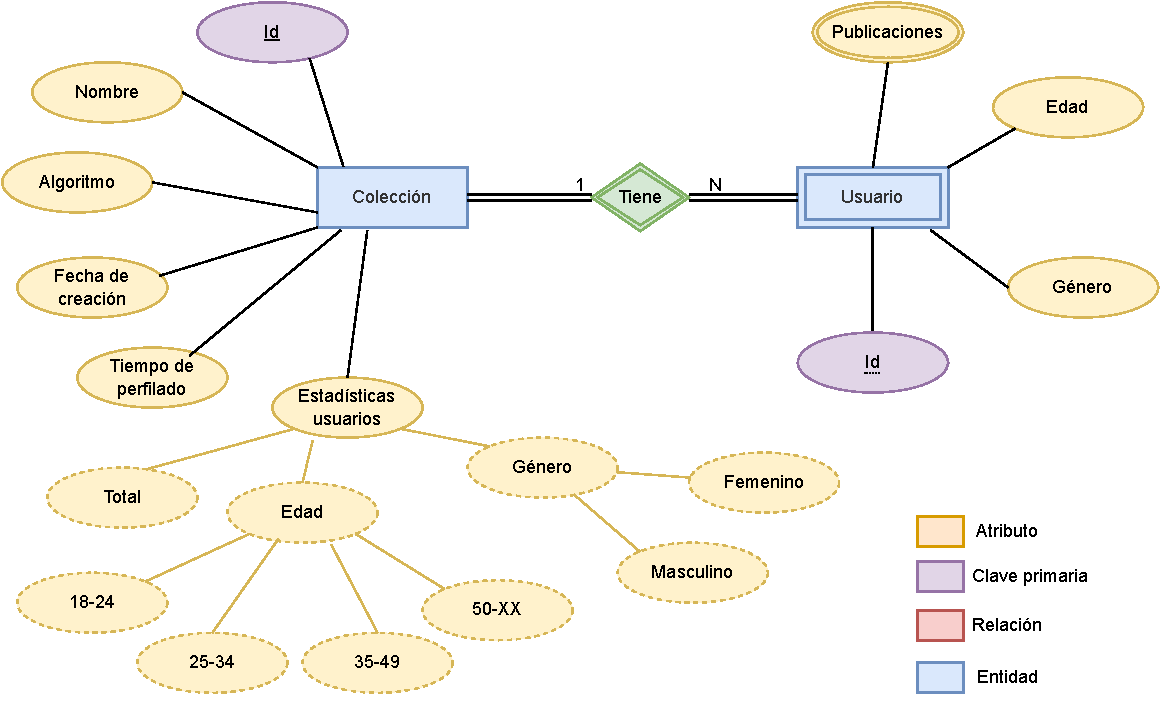
\includegraphics[width=0.95\textwidth]{ER-diagram.pdf}
%			\caption{Diagrama de entidad-relación del sistema.}
			\label{fig:diagrama/ER}
		\end{figure}
	\end{frame}
\subsection{Diseño}

	\begin{frame}
		\frametitle{Diseño}
		\framesubtitle{Arquitectura global}
		Se ha optado por una arquitectura cliente-servidor distribuida en 3 capas.
		\begin{figure}[H]
			\centering
			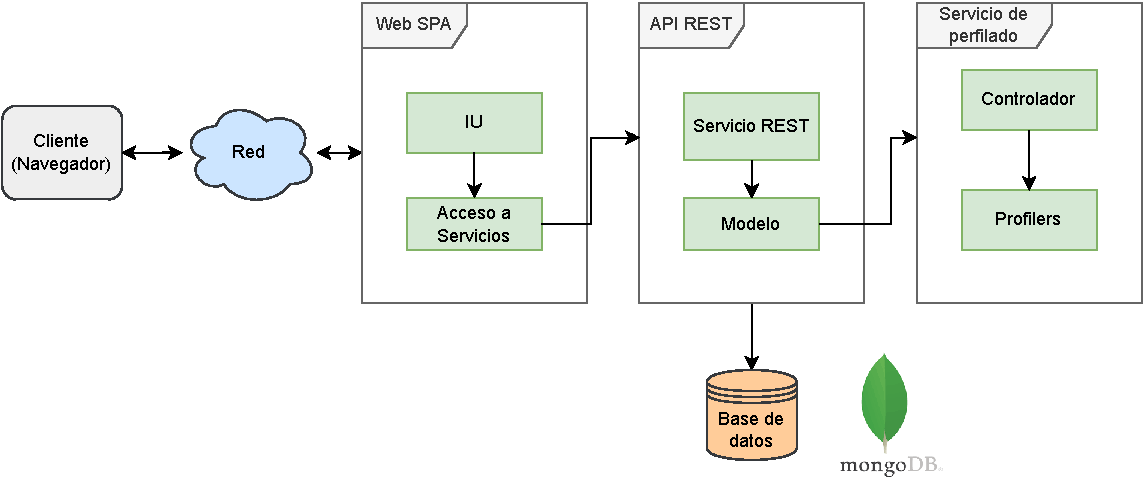
\includegraphics[width=\textwidth]{arquitectura.pdf}
%			\caption{Diagrama de la arquitectura global del sistema.}
			  \label{fig:diagrama/arquitectura}
		\end{figure}
	\end{frame}

\subsection{Desarrollo}
	\begin{frame}
		\frametitle{Desarrollo}
		\framesubtitle{Sprints}

		\begin{enumerate}
			\item Configuración del entorno e investigación del estado del arte (14-3-2023 a 4-4-2023) \pause
			\item Búsqueda, comparación y selección de algoritmos y \textit{datasets} a emplear (4-3-2023 a 25-4-2023) \pause
			\item Primera aproximación y creación de \textit{scraper} para descarga de \textit{dataset} (25-4-2023 a 16-5-2023) \pause
			\item Adaptación de algoritmos restantes y extracción de resultados (20-6-2023 a 11-7-2023) \pause
			\item Desarrollo del micro-servicio de perfilado (11-7-2023 a 1-8-2023) \pause
			\item Inicio del \textit{frontend} y creación de las primeras visualizaciones (1-8-2023 a 21-8-2023) \pause
			\item Lista y detalle de usuarios (21-8-2023 a 11-9-2023) \pause
			\item Persistencia de las colecciones y rediseño del \textit{dashboard} (11-9-2023 a 2-10-2023) \pause
			\item Lista de colecciones y filtrado de usuarios por categoría (2-9-2023 a 23-10-2023) \pause
			%\item Sprint 10: Redacción de la memoria (23-10-2023 6-11-2023)
		\end{enumerate}
	\end{frame}
\section{Análisis corpus \#BLM}

% \begin{frame}
%	\frametitle{Resultados perfilado}
%	\framesubtitle{Algorimto de Modaresi - Edad}
% \begin{figure}[H]
%	\centering
%	\begin{subfigure}{0.2\textwidth}
%		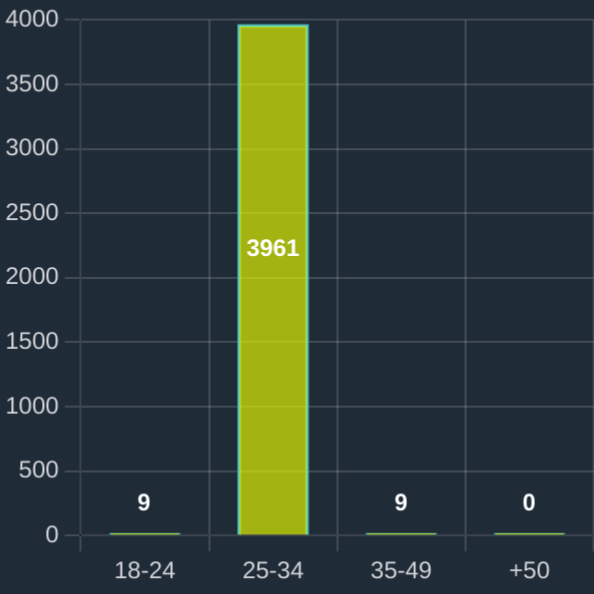
\includegraphics[width=\textwidth]{imaxes/capturas-app/graficos/modaresi/grafico-edad-moda.png}
%		\caption{Total}
%		\label{subfig:blm/resultados-edad-moda}
%	\end{subfigure}
%	\begin{subfigure}{0.2\textwidth}
%		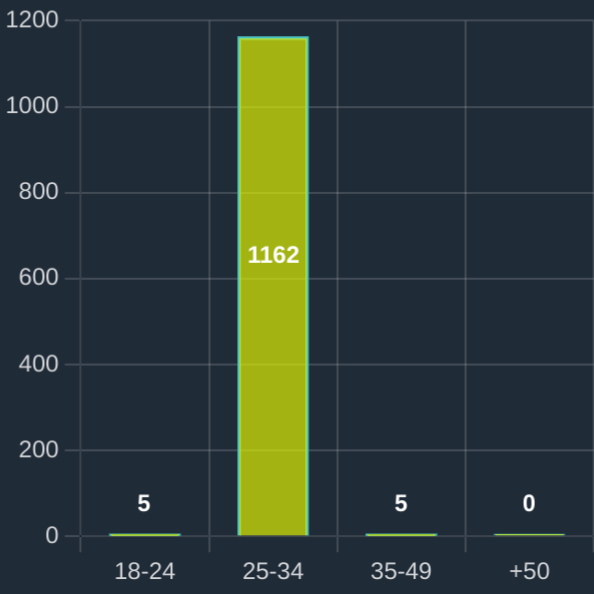
\includegraphics[width=\textwidth]{imaxes/capturas-app/graficos/modaresi/grafico-edad-moda-fem.png}
%		\caption{Usuarios femeninos} 
%	\end{subfigure}
%	\begin{subfigure}{0.18\textwidth}
%		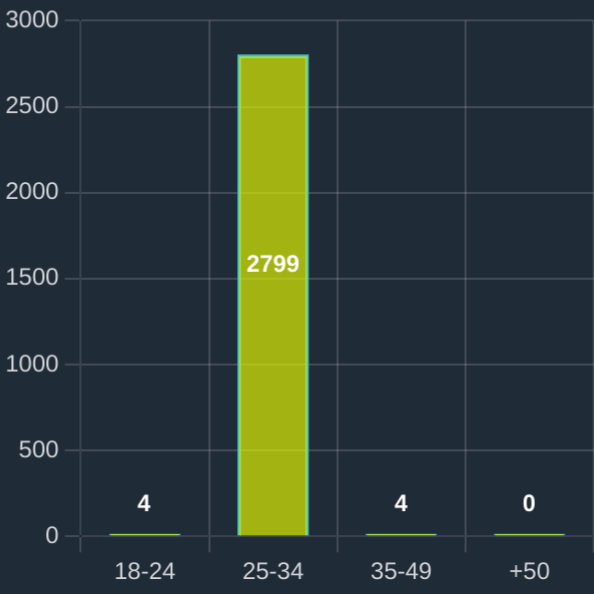
\includegraphics[width=\textwidth]{imaxes/capturas-app/graficos/modaresi/grafico-edad-moda-masc.png}
%		\caption{Usuarios masculinos} 
%	\end{subfigure}
% \end{figure}
%	\begin{figure}[H]
%	\begin{subfigure}{0.18\textwidth}
%		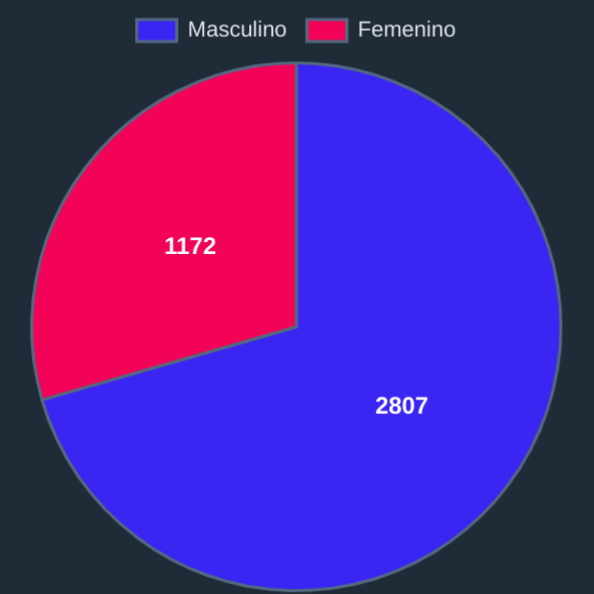
\includegraphics[width=\textwidth]{imaxes/capturas-app/graficos/modaresi/grafico-genero.png}
%		\caption{Total}
%		\label{subfig:blm/resultados-genero-moda}
%	\end{subfigure}
%	\begin{subfigure}{0.18\textwidth}
%		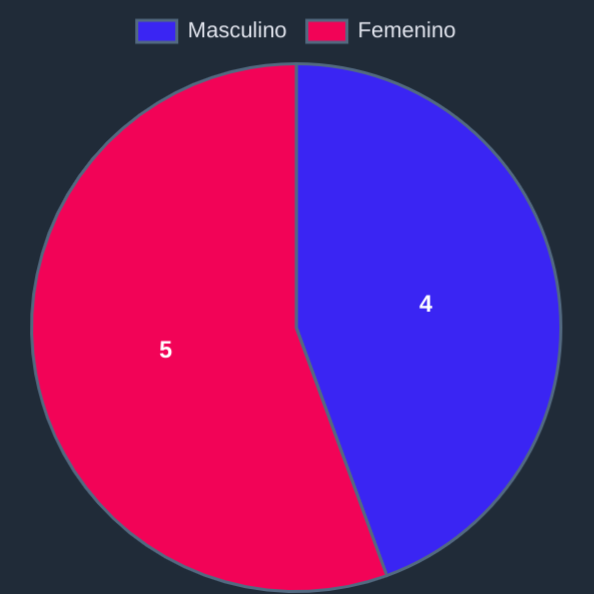
\includegraphics[width=\textwidth]{imaxes/capturas-app/graficos/modaresi/grafico-genero-jj.png}
%		\caption{18-24 años}
%	\end{subfigure}
%	\begin{subfigure}{0.18\textwidth}
%		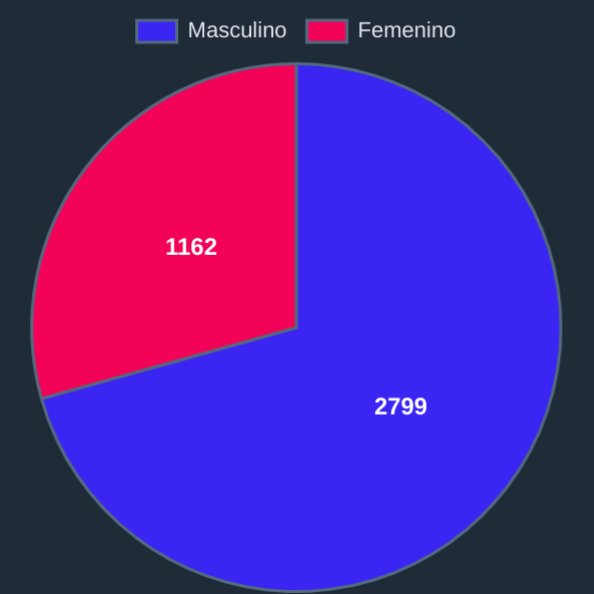
\includegraphics[width=\textwidth]{imaxes/capturas-app/graficos/modaresi/grafico-genero-j.png}
%		\caption{25-34 años}
%	\end{subfigure}
%	\begin{subfigure}{0.18\textwidth}
%		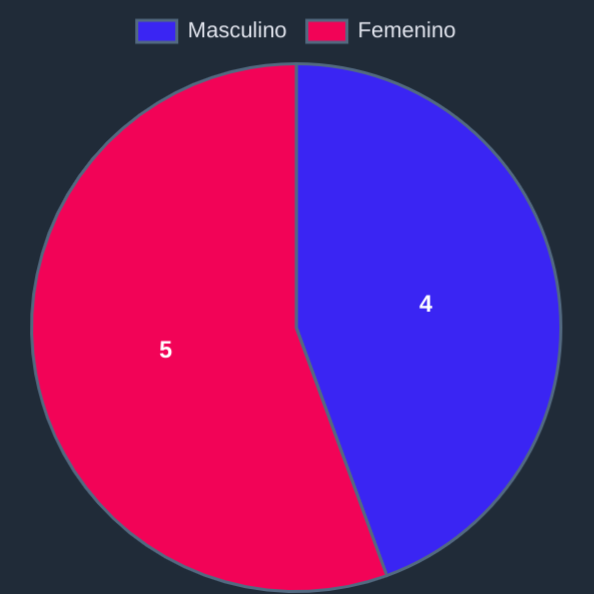
\includegraphics[width=\textwidth]{imaxes/capturas-app/graficos/modaresi/grafico-genero-v.png}
%		\caption{35-49 años}
%	\end{subfigure}
%	\begin{subfigure}{0.18\textwidth}
%		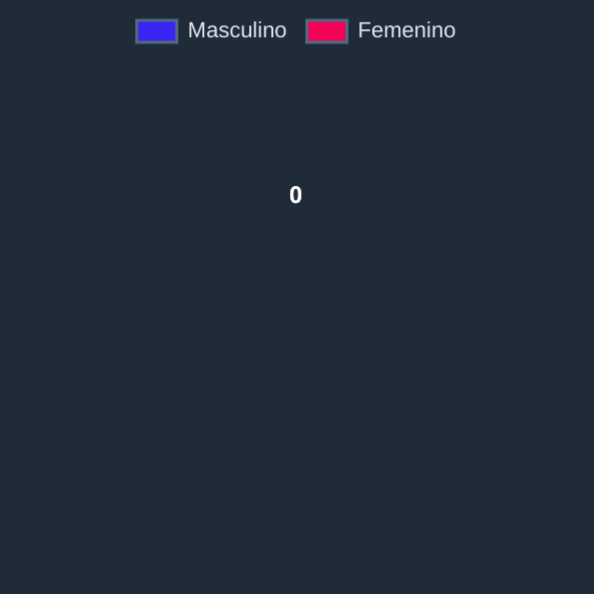
\includegraphics[width=\textwidth]{imaxes/capturas-app/graficos/modaresi/grafico-genero-vv.png}
%		\caption{+50 años}
%	\end{subfigure}
% \end{figure}

% \end{frame}

\subsection{Algoritmo de Grivas}
\begin{frame}
	\frametitle{Resultados perfilado}
	\framesubtitle{Algoritmo de Grivas}
	 \begin{figure}[H]
		\centering
		\begin{subfigure}{0.3\textwidth}
				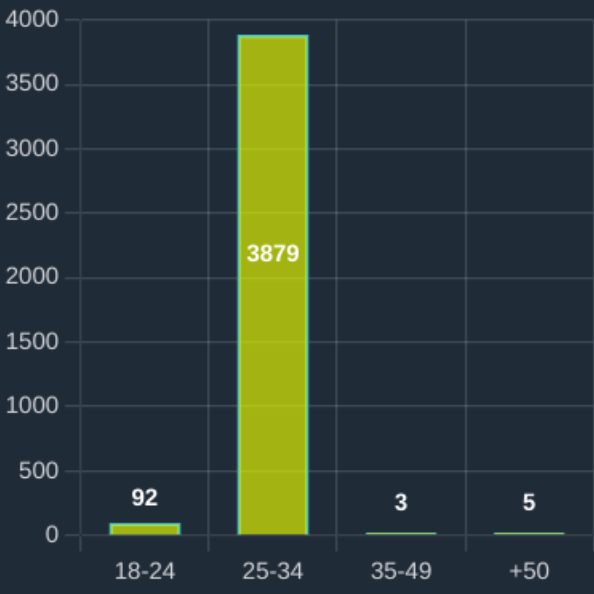
\includegraphics[width=\textwidth]{imaxes/capturas-app/graficos/grivas/grafico-edad-grivas.png}
				\caption{Edad}
				\label{subfig:blm/resultados-edad-moda}
			\end{subfigure}
			\begin{subfigure}{0.3\textwidth}
					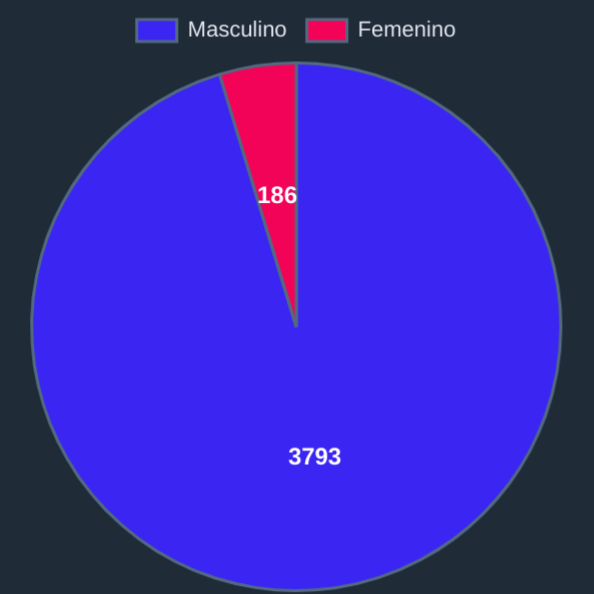
\includegraphics[width=\textwidth]{imaxes/capturas-app/graficos/grivas/grafico-genero.png}
					\caption{Género}
					\label{subfig:blm/resultados-genero-moda}
			\end{subfigure}
		\end{figure}
			\begin{table}[H]
			{
				\setlength{\tabcolsep}{0.6\tabcolsep}
				\begin{tabular}{|c|c|c|c|c|c|}
					\hline
					\diagbox{\textbf{Género}}{\textbf{Edad}} & \textbf{18-24} & \textbf{25-34} & \textbf{35-49} & \textbf{+50} & \textbf{Total} \\ \hline
					\textbf{Femenino} & 31 & 154 & 0 & 1 & 186 \\ \hline
					\textbf{Masculino} & 61 & 3725 & 3 & 4 & 3793 \\ \hline
					\textbf{Total} & 92 & 3879 & 3 & 5 & 3979 \\ \hline
					
				\end{tabular}%
			}
		\end{table}
\end{frame}
\subsection{Algoritmo de Modaresi}
\begin{frame}
	\frametitle{Resultados perfilado}
	\framesubtitle{Algoritmo de Modaresi}
	\begin{figure}[H]
		\centering
		\begin{subfigure}{0.3\textwidth}
			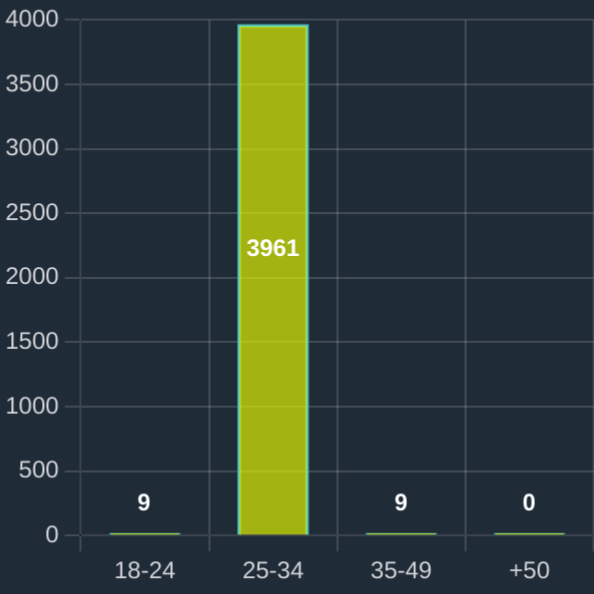
\includegraphics[width=\textwidth]{imaxes/capturas-app/graficos/modaresi/grafico-edad-moda.png}
			\caption{Edad}
			\label{subfig:blm/resultados-edad-moda}
		\end{subfigure}
		\begin{subfigure}{0.3\textwidth}
			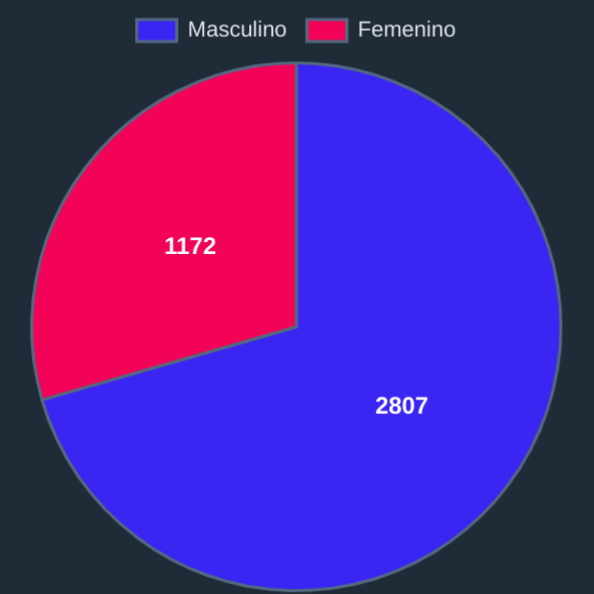
\includegraphics[width=\textwidth]{imaxes/capturas-app/graficos/modaresi/grafico-genero.png}
			\caption{Género}
			\label{subfig:blm/resultados-genero-moda}
		\end{subfigure}
	\end{figure}
	\begin{table}[H]
		\centering
		{
			\setlength{\tabcolsep}{0.6\tabcolsep}
			\begin{tabular}{|c|c|c|c|c|c|}
				\hline
				\diagbox{\textbf{Género}}{\textbf{Edad}} & \textbf{18-24} & \textbf{25-34} & \textbf{35-49} & \textbf{+50} & \textbf{Total} \\ \hline
				\textbf{Femenino} & 5 & 1162 & 5 & 0 & 1172 \\ \hline
				\textbf{Masculino} & 4 & 2799 & 4 & 0 & 2807 \\ \hline
				\textbf{Total} & 9 & 3961 & 9 & 0 & 3979 \\ \hline
				
			\end{tabular}%
		}
	\end{table}
\end{frame}
\subsection{Discusión de resultados}
\begin{frame}
	\frametitle{Resultados perfilado}
	\framesubtitle{Discusión}
	\begin{columns}[T]
		\hspace{-3.5cm}
		\begin{column}{\textwidth}
			\begin{description}[labelwidth=0.01mm]
				\item 
				\vspace{-0.75cm}
				\begin{itemize}
					\item<1->Gran desequilibrio en edad para grupo de 25-34 años ($\impliedby$) desequilibrio entrenamiento 
					\item<3-> Los usuarios varones representan más del 3/4 del corpus.
					\item<4-> Distribución usuarios Reddit $\implies$ distribución corpus.
					\item<5-> 48.98\% corpus tienen menos de 2 publicaciones. El 80\% menos de 5.
					\\ \hspace{2cm}$\downarrow$
					\item <6-> Baja fiabilidad del perfilado que puede acentuar los desequilibrios.
					\item <7-> Preferible a mostrar unos resultados no representativos.
					\item<8->  Resultados similares a corpus inglés: usuarios mayoritariamente varones entre 25-34 años.
				\end{itemize}
			\end{description}
			
		\end{column}
				\hspace{-1.5cm}
			\onslide<2->{
		\begin{column}{0.6\textwidth}

			\vspace{-0.75cm}
			\begin{figure}[H]
				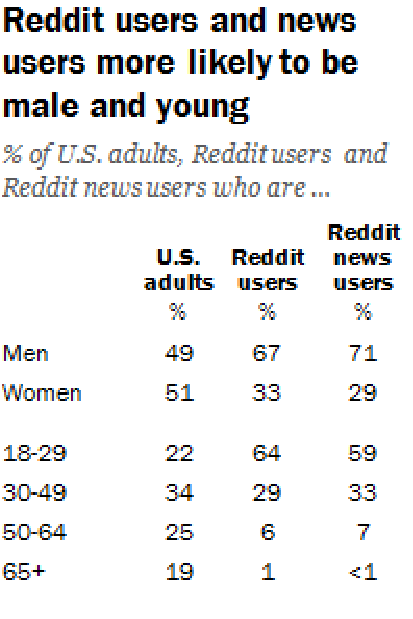
\includegraphics[width=0.5\textwidth]{imaxes/estudio-reddit.pdf}
			\end{figure}
		\end{column}}
	\end{columns}
\end{frame}

\section{Conclusiones}

	\begin{frame}
			\frametitle{Conclusiones}
			\framesubtitle{Evaluación estado actual y lecciones aprendidas}
			\vspace{0cm}
			\textbf{Resultados:}
			\begin{itemize}
				\item Se exploraron y probaron varios algoritmos del estado del arte del perfilado automático de usuarios con buen rendimiento.
				\item Se creó una herramienta mediante unas buenas prácticas de ingeniería que a la vez es escalable, extensible y portable con una interfaz intuitiva y accesible.
				\item Se analizó el corpus de referencia sobre \#BLM de forma satisfactoria. 

			\end{itemize} 
			\pause
			\vspace{0.5cm}
			\textbf{Lecciones aprendidas:}
			\begin{itemize}
				\item Importancia del seguimiento de unas pautas metodológicas estrictas (primera fase).
				\item Conocimientos que se valoraron en retrospectiva y asentaron gracias a este proyecto.
				\item Perspectiva mucho más amplia de mis posibilidades en esta profesión.
			\end{itemize}
	\end{frame}
	
	\begin{frame}
		\frametitle{Trabajo futuro}
		\vspace{-2cm}
%		Dos líneas:
		\vspace{1cm}
		\begin{columns}[T]
			\hspace{-3.5cm}

			\begin{column}{0.8\textwidth}
			\vspace{-1cm}
				\begin{description}[labelwidth=0.01mm]
					\item \textbf{Mejora algoritmos perfilado}
					\begin{itemize}
						\item Aumento tamaño y calidad corpus entrenamiento. \pause
						\item Uso de algoritmos de clasificación basados en \textit{transformers} como LLM. \pause
						\item Perfilado sobre rasgos de personalidad, nivel de vida, educación...
						
						\end{itemize}
				\end{description}
			\end{column}
			\hspace{-3.5cm}

			\begin{column}{0.8\textwidth}
							\vspace{-1cm}
				\begin{description}[labelwidth=0.01mm]
					\item \textbf{Ampliación funcionalidad:}
					\begin{itemize}
						\item Perfilado de forma asíncrona por parte del usuario. \pause
						\item Exportar datos del \textit{dashboard}, incluyendo gráficos y visualizaciones.\pause
						\item Visualización de características de escritura en \textit{dashboard} sobre usuarios perfilados.
						
					\end{itemize}
				\end{description}
			\end{column}
		\end{columns}
	\end{frame}
	
\begin{frame}[plain]
	\begin{center}
		\Huge ¡Gracias por su atención!
	\end{center}
\end{frame}

\end{document}